%%%%%%%% NeurIPS 2025 STYLE %%%%%%%%%%%%%%%%%

\documentclass{article}

\usepackage[preprint]{neurips_2025}

\usepackage[utf8]{inputenc}
\usepackage[T1]{fontenc}
\usepackage{hyperref}
\usepackage{url}
\usepackage{booktabs}
\usepackage{amsfonts}
\usepackage{nicefrac}
\usepackage{microtype}
\usepackage{graphicx}
\usepackage{subcaption}
\usepackage{amsmath}
\usepackage{amssymb}
\usepackage{mathtools}
\usepackage{amsthm}
\usepackage[capitalize,noabbrev]{cleveref}
\usepackage{xcolor}
\usepackage{multirow}
\usepackage{tikz}
\usetikzlibrary{arrows.meta,positioning,shapes.geometric,calc,fit}

\raggedbottom

\title{The Shape of Wisdom, Part~I:\\
Decision-Space Dynamics from Cached Layerwise Option Scores}

\author{%
  \textbf{Shailesh Rana} \\
  Independent Researcher \\
}

\makeatletter
\renewcommand{\@notice}{}
\makeatother

\begin{document}

\twocolumn[
\begin{@twocolumnfalse}
\maketitle

%% ============================================================
%% ABSTRACT
%% ============================================================
\begin{abstract}
When a transformer answers a multiple-choice question, its preference among the four options evolves layer by layer.
We study this evolution across three 7--8\,B instruction-tuned models (Qwen~2.5-7B, Llama~3.1-8B, Mistral~7B-v0.3) using \emph{only} cached per-layer option scores---no new inference is performed.
We define a soft margin~$\delta_{\mathrm{soft}}$ that smooths competitor-switching artifacts via a temperature-scaled log-sum-exp over incorrect options, and use it to classify 9{,}000 model--prompt pairs into three regimes---\emph{Stable-Correct}, \emph{Stable-Wrong}, and \emph{Unstable}.
In a four-dimensional ``decision space'' whose axes are the four option scores, PCA reveals coherent trajectory bundles that separate by regime.
A flow field computed over normalised depth and soft margin shows convergent drift toward the decision boundary from above and below, with late-layer commitment concentrating in the final 20--30\% of depth.
Robustness analysis across temperature $\tau \in \{0.5, 1.0, 2.0\}$ and commitment threshold $M \in \{0.5, 0.75, 1.0\}$ confirms that regime proportions shift smoothly rather than discontinuously.
All results derive from cached four-option logit vectors; we make no mechanistic claims about internal attention or MLP circuits.
\end{abstract}
\vspace{0.2cm}
\end{@twocolumnfalse}
]

%% ============================================================
%% 1. INTRODUCTION
%% ============================================================
\section{Introduction}
\label{sec:intro}

A transformer answering a four-choice question does not make a single decision.
At each layer, the output distribution over the four answer tokens shifts---sometimes toward the correct answer, sometimes away from it.
By the final layer, the model has committed.
What happens in between is what this paper is about.

Prior work has studied transformer internals through probing classifiers~\cite{belinkov2022}, causal tracing~\cite{meng2022}, and circuit-level analysis~\cite{olsson2022,conmy2023}.
These methods typically require running the model, injecting perturbations, or training auxiliary networks.
We take a complementary approach: given a cache of per-layer logit scores for four answer options, \emph{what can we learn about how a model decides?}

Our answer is structured around three ideas.
First, we define a \emph{soft margin}~$\delta_{\mathrm{soft}}$ that pools all incorrect options into a single competitor signal via log-sum-exp, avoiding the jagged artifacts that arise when the identity of the strongest competitor switches between layers.
Second, we classify model--prompt pairs into three regimes (Stable-Correct, Stable-Wrong, Unstable) based on the trajectory of $\delta_{\mathrm{soft}}$ across depth, quantifying commitment and instability without overclaiming sharp phase transitions.
Third, we construct a ``decision space'' by treating the four option scores as coordinates and visualising trajectories via PCA---making explicit that this is a proxy space defined by the four-option readout, not the full hidden-state space.

\paragraph{Contributions.}
\begin{enumerate}
\item A soft-margin definition that resolves competitor-switching artifacts inherent in hard-max margins (\cref{sec:definitions}).
\item A regime classification with measurable commitment depth and flip count, replicated across three architectures (\cref{sec:findings}).
\item Decision-space visualizations (PCA trajectories, flow fields) that reveal convergent structure without requiring hidden-state access (\cref{sec:findings}).
\item Robustness analysis demonstrating smooth degradation under hyperparameter perturbation (\cref{sec:robustness}).
\end{enumerate}

All results derive from cached artifacts.
No new model inference was performed.
The analysis code, canonical data table, and reproducibility stamp are available in the supplementary material.


%% ============================================================
%% 2. DEFINITIONS
%% ============================================================
\section{Definitions}
\label{sec:definitions}

We study four-choice (A/B/C/D) questions.  At each transformer layer $l \in \{0, \ldots, L{-}1\}$, we extract logit scores for the four answer tokens via a token-bucket readout~\cite{nostalgebraist2020} and work exclusively in this four-dimensional subspace.

\subsection{Score vectors and correct option}

Let $s_A(l), s_B(l), s_C(l), s_D(l)$ denote the four option scores at layer $l$, and let $c$ denote the correct option (ground-truth answer key).
The score vector at layer $l$ is $\mathbf{v}(l) = [s_A(l),\, s_B(l),\, s_C(l),\, s_D(l)]$.

\subsection{Competitor definitions}

We define three notions of ``competitor.''

\paragraph{Dynamic competitor.}
At each layer, the strongest incorrect option:
\begin{equation}
  k_{\mathrm{dyn}}(l) = \arg\max_{j \neq c}\; s_j(l).
  \label{eq:k_dyn}
\end{equation}
Ties are broken by alphabetical order (A~$<$~B~$<$~C~$<$~D).

\paragraph{Fixed competitor.}
The dynamic competitor at the final layer:
\begin{equation}
  k_{\mathrm{fix}} = k_{\mathrm{dyn}}(L{-}1).
  \label{eq:k_fix}
\end{equation}

\paragraph{Soft competitor.}
A temperature-scaled aggregation of all incorrect options:
\begin{equation}
  \mathrm{softcomp}_\tau(l) = \tau \cdot \mathrm{logsumexp}_{j \neq c}\!\left(\frac{s_j(l)}{\tau}\right).
  \label{eq:softcomp}
\end{equation}

\subsection{Margin definitions}
\label{sec:margins}

\paragraph{Hard dynamic margin.}
\begin{equation}
  \delta_{\mathrm{hard,dyn}}(l) = s_c(l) - \max_{j \neq c}\, s_j(l).
  \label{eq:delta_hard_dyn}
\end{equation}

\paragraph{Hard fixed margin.}
\begin{equation}
  \delta_{\mathrm{hard,fix}}(l) = s_c(l) - s_{k_\mathrm{fix}}(l).
  \label{eq:delta_hard_fix}
\end{equation}

\paragraph{Soft margin.}
\begin{equation}
  \delta_{\mathrm{soft}}(l;\tau) = s_c(l) - \mathrm{softcomp}_\tau(l).
  \label{eq:delta_soft}
\end{equation}

\textbf{Default margin.}  Throughout this paper, $\delta \equiv \delta_{\mathrm{soft}}(\cdot\,; \tau{=}1.0)$ unless stated otherwise.

\emph{Why soft?}  The hard dynamic margin~$\delta_{\mathrm{hard,dyn}}$ can exhibit sharp jumps when the identity of the strongest incorrect option changes between layers---a \emph{competitor switch}.
The soft margin pools all competitors smoothly, producing a trajectory that reflects the correct option's overall advantage rather than its lead over a single, possibly switching, contender.
The temperature $\tau$ controls the softness: at $\tau \to 0$, $\delta_{\mathrm{soft}}$ converges to $\delta_{\mathrm{hard,dyn}}$; at large $\tau$, it converges to $s_c - \bar{s}_{\mathrm{incorrect}}$.

\subsection{Derived quantities}

\paragraph{Competitor switching.}
\begin{equation}
  \mathrm{switch}(l) = \mathbb{1}\bigl[l \geq 1 \;\wedge\; k_{\mathrm{dyn}}(l) \neq k_{\mathrm{dyn}}(l{-}1)\bigr].
  \label{eq:switch}
\end{equation}

\paragraph{Final sign and signed margin.}
Let $\mathrm{sign}_{\mathrm{final}} = \mathrm{sign}(\delta(L{-}1))$.
The signed margin is $\delta_{\mathrm{signed}}(l) = \mathrm{sign}_{\mathrm{final}} \cdot \delta(l)$, aligning every trajectory so that the final decision points upward.

\paragraph{Flip count.}
Compute the sign sequence of $\delta$ across layers, dropping exact zeros.
The flip count is the number of sign changes in this sequence.

\paragraph{Commitment layer~$\ell^*$.}
The smallest $l$ such that $\delta_{\mathrm{signed}}(l') \geq M$ for all $l' \geq l$, where we set $M = 0.75$ by default.
If no such $l$ exists, $\ell^* = \varnothing$.

\paragraph{Normalised depth.}
$d = l / (L{-}1) \in [0, 1]$.

\subsection{Regime classification}
\label{sec:regimes}

A model--prompt pair is classified into one of three regimes:
\begin{itemize}
\item \textbf{Stable-Correct.}  Flip count $\leq 1$, commitment layer exists, and $\delta(L{-}1) > 0$.
\item \textbf{Stable-Wrong.}  Flip count $\leq 1$, commitment layer exists, and $\delta(L{-}1) < 0$.
\item \textbf{Unstable.}  All other cases (too many flips, no commitment, or $\delta(L{-}1) = 0$).
\end{itemize}
This classification is a convention---a useful partition whose boundaries shift smoothly under hyperparameter perturbation (\cref{sec:robustness}).
We do not claim a natural discontinuity between regimes.


%% ============================================================
%% FIGURE 0: PIPELINE SCHEMATIC (TikZ)
%% ============================================================
\begin{figure*}[t]
\vskip 0.1in
\begin{center}
\resizebox{0.95\textwidth}{!}{%
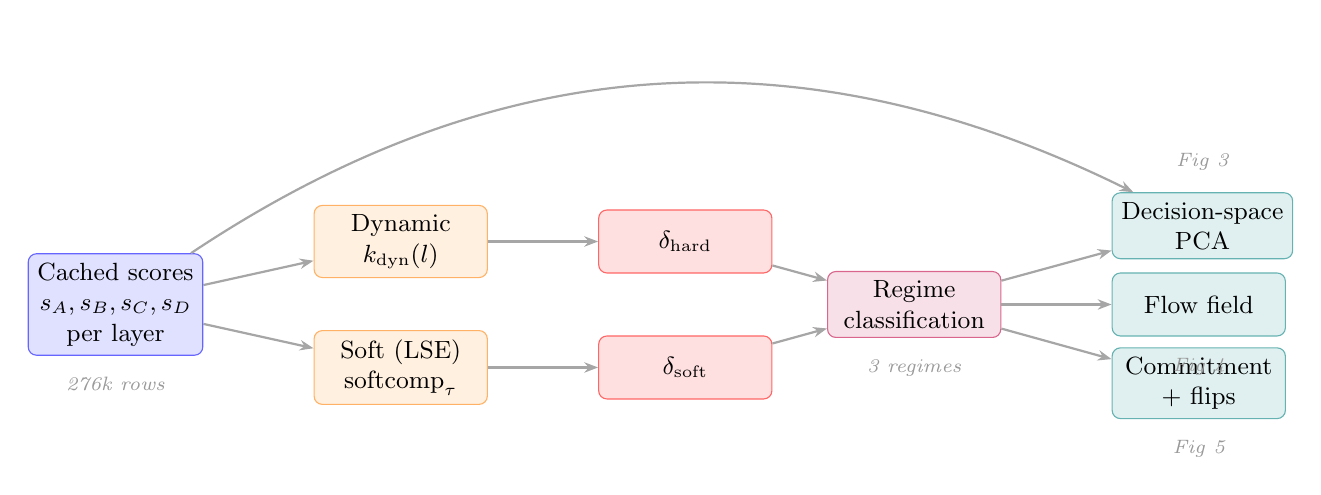
\begin{tikzpicture}[
    box/.style={draw, rounded corners=3pt, minimum width=2.2cm, minimum height=0.8cm,
                font=\small, align=center, fill=#1!12, draw=#1!60},
    box/.default=blue,
    arrow/.style={-{Stealth[length=5pt]}, thick, draw=gray!70},
    label/.style={font=\scriptsize\itshape, text=gray!80},
]
% Input
\node[box=blue] (input) {Cached scores\\$s_A, s_B, s_C, s_D$\\per layer};

% Competitor modes
\node[box=orange, right=1.4cm of input, yshift=0.8cm] (dyn) {Dynamic\\$k_{\mathrm{dyn}}(l)$};
\node[box=orange, right=1.4cm of input, yshift=-0.8cm] (soft) {Soft (LSE)\\$\mathrm{softcomp}_\tau$};

% Margins
\node[box=red, right=1.4cm of dyn] (delta_hard) {$\delta_{\mathrm{hard}}$};
\node[box=red, right=1.4cm of soft] (delta_soft) {$\delta_{\mathrm{soft}}$};

% Regime
\node[box=purple, right=1.8cm of $(delta_hard)!0.5!(delta_soft)$] (regime) {Regime\\classification};

% Analyses
\node[box=teal, right=1.4cm of regime, yshift=1.0cm] (pca) {Decision-space\\PCA};
\node[box=teal, right=1.4cm of regime, yshift=-0.0cm] (flow) {Flow field};
\node[box=teal, right=1.4cm of regime, yshift=-1.0cm] (commit) {Commitment\\+ flips};

% Arrows
\draw[arrow] (input) -- (dyn);
\draw[arrow] (input) -- (soft);
\draw[arrow] (dyn) -- (delta_hard);
\draw[arrow] (soft) -- (delta_soft);
\draw[arrow] (delta_hard) -- (regime);
\draw[arrow] (delta_soft) -- (regime);
\draw[arrow] (regime) -- (pca);
\draw[arrow] (regime) -- (flow);
\draw[arrow] (regime) -- (commit);
\draw[arrow] (input) to[bend left=30] (pca);

% Labels
\node[label, below=0.15cm of input] {276k rows};
\node[label, below=0.15cm of regime] {3 regimes};
\node[label, above=0.15cm of pca] {Fig~3};
\node[label, below=0.15cm of flow] {Fig~4};
\node[label, below=0.15cm of commit] {Fig~5};
\end{tikzpicture}
}
\caption{Pipeline overview.
Cached per-layer option scores for three models flow through competitor definitions and margin computations into regime classification and three downstream analyses.
All computations use only the four cached logit scores per layer; no hidden states or model weights are accessed.}
\label{fig:pipeline}
\end{center}
\end{figure*}


%% ============================================================
%% 3. FINDINGS
%% ============================================================
\section{Findings}
\label{sec:findings}

We analyse 9{,}000 model--prompt pairs (3 models $\times$ 3{,}000 MMLU questions).
All figures show $\delta_{\mathrm{soft}}(\tau{=}1.0)$ unless noted.

\subsection{Example trajectories}
\label{sec:examples}

\cref{fig:examples} shows representative margin trajectories for each regime.
Stable-Correct trajectories rise monotonically or with minor fluctuations, crossing above the commitment threshold $M = 0.75$ before the final quarter of depth.
Stable-Wrong trajectories mirror this pattern below zero, with the signed margin $\delta_{\mathrm{signed}}$ exceeding $M$ in the wrong-answer direction.
Unstable trajectories oscillate across the zero boundary, sometimes recovering and sometimes not.

\begin{figure*}[t]
\vskip 0.1in
\begin{center}
\centerline{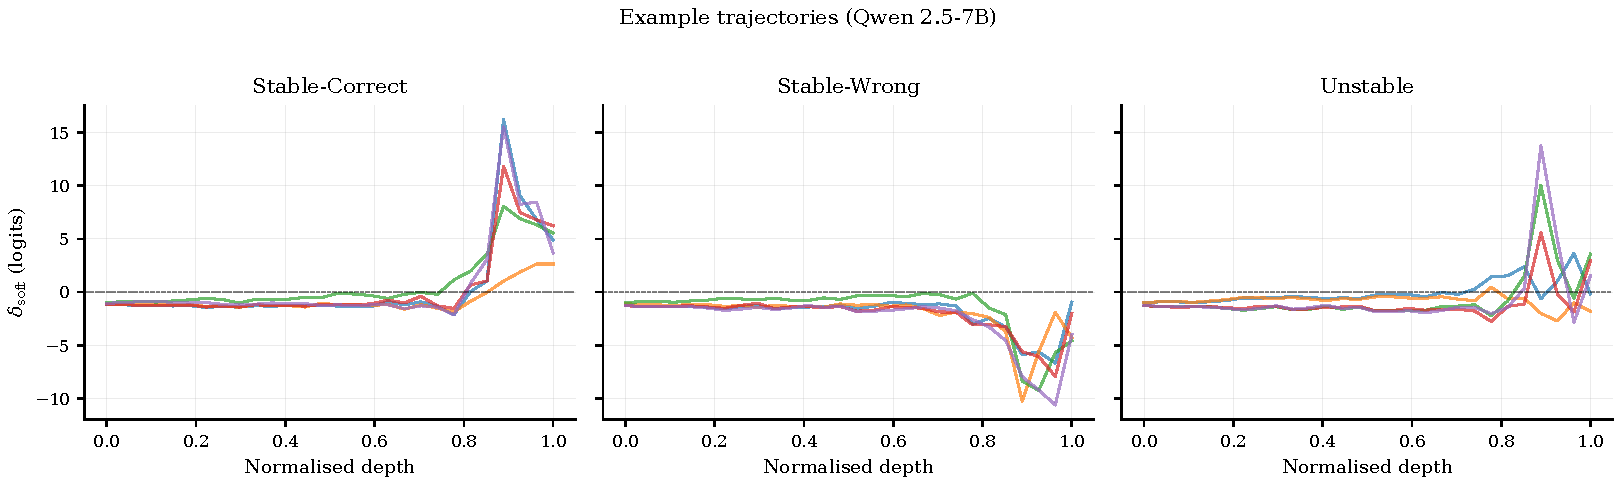
\includegraphics[width=0.95\textwidth]{figures/fig1_examples.pdf}}
\caption{Soft-margin trajectories reveal three distinct decision patterns.
Five randomly sampled trajectories per regime for Qwen~2.5-7B, plotted as $\delta_{\mathrm{soft}}(\tau{=}1)$ versus normalised depth.
Stable-Correct trajectories converge above zero; Stable-Wrong trajectories converge below; Unstable trajectories oscillate near the boundary.}
\label{fig:examples}
\end{center}
\end{figure*}

\subsection{Margin distributions across depth}
\label{sec:distributions}

\cref{fig:distributions} presents the distribution of $\delta_{\mathrm{soft}}$ at five depth slices.
At depth 0 (embedding), all three regimes overlap near zero---no regime is separable.
By depth 0.5, Stable-Correct and Stable-Wrong have begun to diverge.
By depth 1.0 (final layer), the three regimes occupy non-overlapping regions.

The pattern replicates across all three models, though absolute magnitudes differ: Qwen produces larger $|\delta|$ than Mistral, reflecting model-specific scaling.

\begin{figure*}[t]
\vskip 0.1in
\begin{center}
\centerline{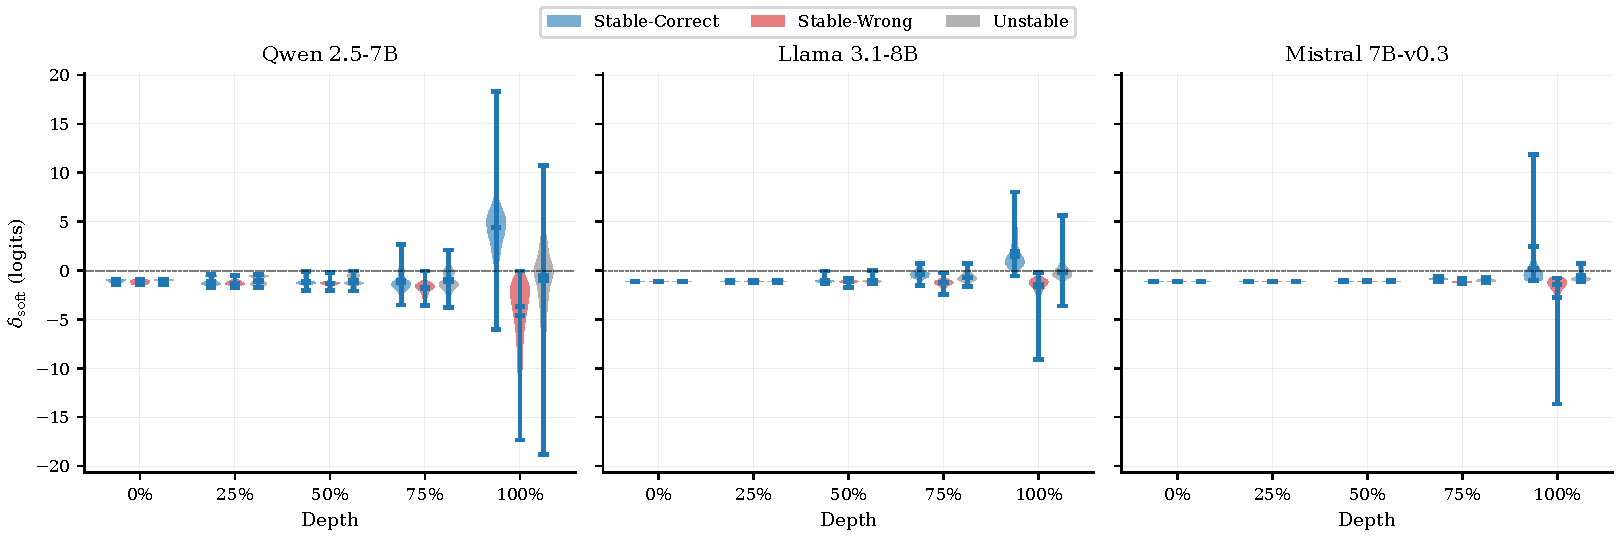
\includegraphics[width=0.95\textwidth]{figures/fig2_delta_distribution.pdf}}
\caption{Regime separation emerges across depth.
Violin plots of $\delta_{\mathrm{soft}}(\tau{=}1)$ at five normalised-depth slices (0\%, 25\%, 50\%, 75\%, 100\%) for each model, coloured by regime.
At depth~0, regimes overlap; by depth~1, they are well separated.
Absolute magnitudes are model-dependent.}
\label{fig:distributions}
\end{center}
\end{figure*}

\subsection{Regime proportions}

\cref{tab:regimes} reports regime counts per model.
Stable-Correct is the majority regime (50--65\% of prompts), consistent with overall model accuracy on MMLU.
Stable-Wrong accounts for 10--20\%, and Unstable for 20--35\%.
Median final $\delta$ confirms that stable regimes satisfy the expected sign.

\begin{table}[t]
  \caption{Regime counts and median final margin $\delta_{\mathrm{soft}}(\tau{=}1)$ per model.}
  \label{tab:regimes}
  \vskip 0.1in
  \begin{center}
  \begin{small}
  \begin{tabular}{llrrl}
    \toprule
    Model & Regime & $N$ & \% & Med.\ $\delta$ \\
    \midrule
    Qwen 2.5-7B & Stable-Correct & 1,590 & 53.0 & +4.05 \\
    Qwen 2.5-7B & Stable-Wrong & 528 & 17.6 & -2.90 \\
    Qwen 2.5-7B & Unstable & 882 & 29.4 & -0.32 \\
    \midrule
    Llama 3.1-8B & Stable-Correct & 1,045 & 34.8 & +3.02 \\
    Llama 3.1-8B & Stable-Wrong & 1,017 & 33.9 & -1.47 \\
    Llama 3.1-8B & Unstable & 938 & 31.3 & +0.00 \\
    \midrule
    Mistral 7B-v0.3 & Stable-Correct & 1,423 & 47.4 & +5.66 \\
    Mistral 7B-v0.3 & Stable-Wrong & 1,247 & 41.6 & -3.75 \\
    Mistral 7B-v0.3 & Unstable & 330 & 11.0 & -0.09 \\
    \bottomrule
  \end{tabular}
  \end{small}
  \end{center}
\end{table}


\subsection{Decision-space trajectories}
\label{sec:pca}

The four option scores define a four-dimensional ``decision space.''
We emphasise that this is \emph{not} the model's internal hidden-state space; it is a proxy defined by the four-token readout.
We use ``decision space'' to distinguish it from the high-dimensional latent representation.

\cref{fig:pca} shows PCA projections of $\mathbf{v}(l) = [s_A, s_B, s_C, s_D]$ for each model.
Trajectories (paths through layers, shown as translucent lines) form coherent bundles by regime.
Final-layer points cluster by regime in the first two principal components, which together explain 60--80\% of variance---unsurprisingly high for a four-dimensional space.

\begin{figure*}[t]
\vskip 0.1in
\begin{center}
\centerline{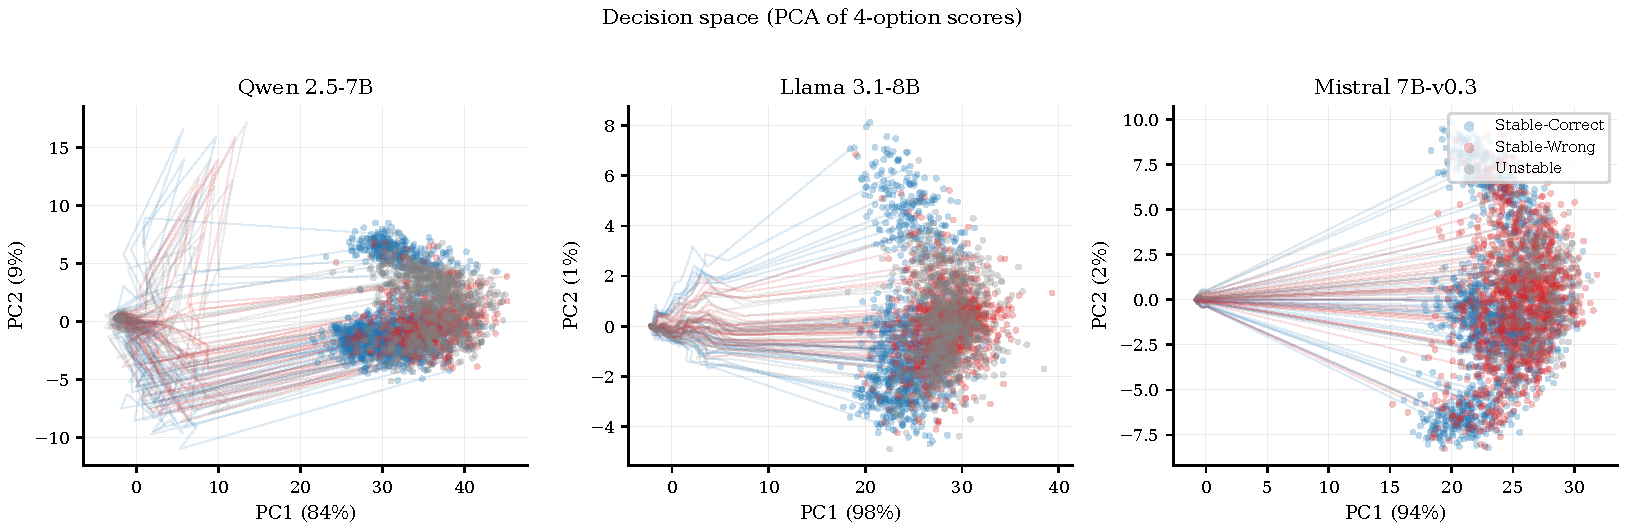
\includegraphics[width=0.95\textwidth]{figures/fig3_decision_space_trajectories.pdf}}
\caption{Trajectories in decision space form regime-coherent bundles.
PCA of the four-option score vector $[s_A, s_B, s_C, s_D]$ across all layers, one panel per model.
Translucent lines trace sampled trajectories through depth; dots mark final-layer positions.
This is a proxy ``decision space'' defined by the four-token readout, not the hidden-state latent space.}
\label{fig:pca}
\end{center}
\end{figure*}

\subsection{Flow field}
\label{sec:flow}

To visualise the aggregate dynamics, we bin the (normalised depth, $\delta_{\mathrm{soft}}$) plane and compute the mean per-layer change in $\delta$ within each bin (\cref{fig:flow}).
The resulting flow field reveals:
\begin{itemize}
\item \emph{Convergence toward zero at early depth}---scores are uninformed and drift is noisy.
\item \emph{Divergence away from zero at mid-depth}---the model begins to commit.
\item \emph{Strong convergence toward the signed final value at late depth}---commitment solidifies.
\end{itemize}

A boundary band (shaded, $|\delta| < 0.2$) highlights the region where decisions are most fragile.
Cells with fewer than 5 observations are masked.

\begin{figure}[t]
\vskip 0.1in
\begin{center}
\centerline{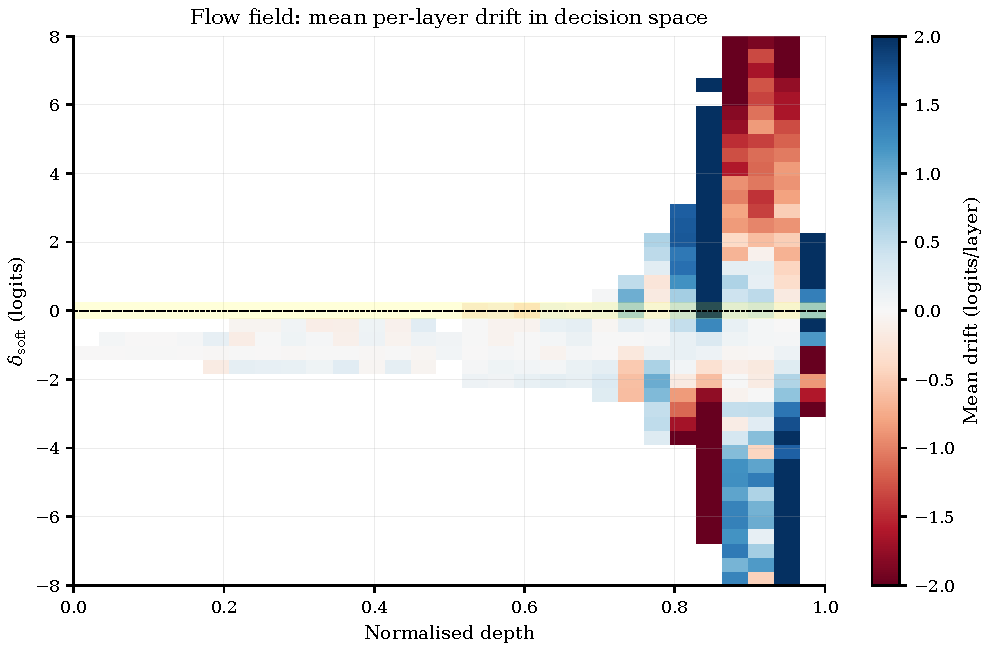
\includegraphics[width=\columnwidth]{figures/fig4_flow_field.pdf}}
\caption{The flow field reveals convergent decision dynamics.
Mean per-layer drift in $\delta_{\mathrm{soft}}$ within bins of normalised depth and clipped margin ($\delta \in [-8, 8]$), pooled across all three models.
Blue: positive drift (toward correct answer); red: negative drift.
Yellow band marks $|\delta| < 0.2$ (decision boundary).
Cells with count $< 5$ are masked.}
\label{fig:flow}
\end{center}
\end{figure}

\subsection{Commitment and instability}
\label{sec:commitment}

\cref{fig:commitment} quantifies four aspects of decision dynamics.
\textbf{(A)}~Commitment depth concentrates in the final 20--30\% of the network for all three models, with Qwen committing slightly earlier.
\textbf{(B)}~Flip counts follow a heavy-tailed distribution: most trajectories have zero or one flip, with Unstable prompts contributing the tail.
\textbf{(C)}~For Unstable prompts, the last sign flip concentrates in the final third of depth, suggesting that late-layer processing is the primary source of instability.
\textbf{(D)}~The competitor switch rate peaks at mid-depth and declines toward the output layer as the model locks onto a competitor.

\begin{figure*}[t]
\vskip 0.1in
\begin{center}
\centerline{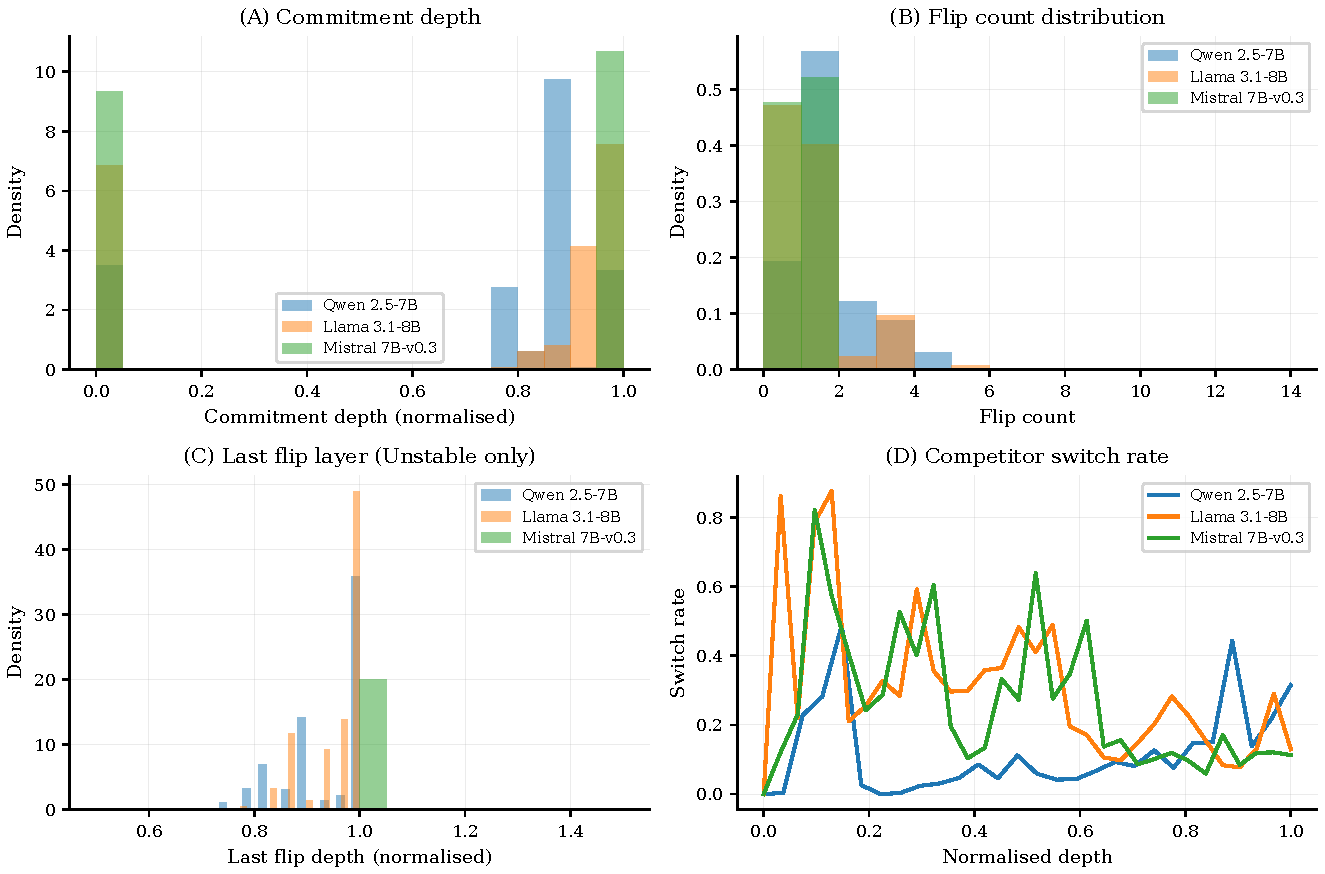
\includegraphics[width=0.95\textwidth]{figures/fig5_commitment_and_flips.pdf}}
\caption{Commitment concentrates late and instability peaks at mid-to-late depth.
\textbf{(A)}~Commitment depth distribution (normalised).
\textbf{(B)}~Flip count histogram.
\textbf{(C)}~Last flip layer for Unstable prompts.
\textbf{(D)}~Competitor switch rate versus normalised depth.
All three models shown; $\delta = \delta_{\mathrm{soft}}(\tau{=}1)$, $M = 0.75$.}
\label{fig:commitment}
\end{center}
\end{figure*}


%% ============================================================
%% 4. ROBUSTNESS
%% ============================================================
\section{Robustness}
\label{sec:robustness}

We verify that the regime structure is not an artifact of our particular hyperparameter choices by varying both the temperature $\tau$ and the commitment threshold $M$.

\cref{fig:robustness} shows regime proportions under $\tau \in \{0.5, 1.0, 2.0\}$ and $M \in \{0.5, 0.75, 1.0\}$, separately for each model.
Two patterns emerge.
First, higher $\tau$ (softer margins) produces slightly fewer Stable classifications as the margin signal is diluted.
Second, higher $M$ (stricter commitment) shifts prompts from Stable to Unstable, as expected.
Crucially, the transitions are smooth: no parameter combination produces a discontinuous jump in regime proportions.

\cref{tab:robustness} reports the pooled (all models) proportions.
Even at the most permissive setting ($\tau = 0.5$, $M = 0.5$), the Unstable class retains a substantial fraction.
Even at the most restrictive ($\tau = 2.0$, $M = 1.0$), the Stable-Correct class is non-trivial.
This smooth variation is what we would expect from a continuous underlying distribution rather than a sharp phase boundary.

\begin{table}[t]
  \caption{Regime proportions (\%) under varying temperature $\tau$ and commitment threshold $M$.
  All three models pooled.}
  \label{tab:robustness}
  \vskip 0.1in
  \begin{center}
  \begin{small}
  \begin{tabular}{ccrrrr}
    \toprule
    $\tau$ & $M$ & Stable-Corr & Stable-Wrong & Unstable \\
    \midrule
    0.5 & 0.50 & 38.9 & 29.0 & 32.1 \\
    0.5 & 0.75 & 37.2 & 26.5 & 36.3 \\
    0.5 & 1.00 & 35.8 & 23.9 & 40.3 \\
    1.0 & 0.50 & 46.5 & 33.7 & 19.9 \\
    1.0 & 0.75 & 45.1 & 31.0 & 23.9 \\
    1.0 & 1.00 & 43.7 & 27.8 & 28.5 \\
    2.0 & 0.50 & 39.2 & 43.7 & 17.1 \\
    2.0 & 0.75 & 37.4 & 41.6 & 21.0 \\
    2.0 & 1.00 & 35.8 & 39.4 & 24.8 \\
    \bottomrule
  \end{tabular}
  \end{small}
  \end{center}
\end{table}


\begin{figure*}[t]
\vskip 0.1in
\begin{center}
\centerline{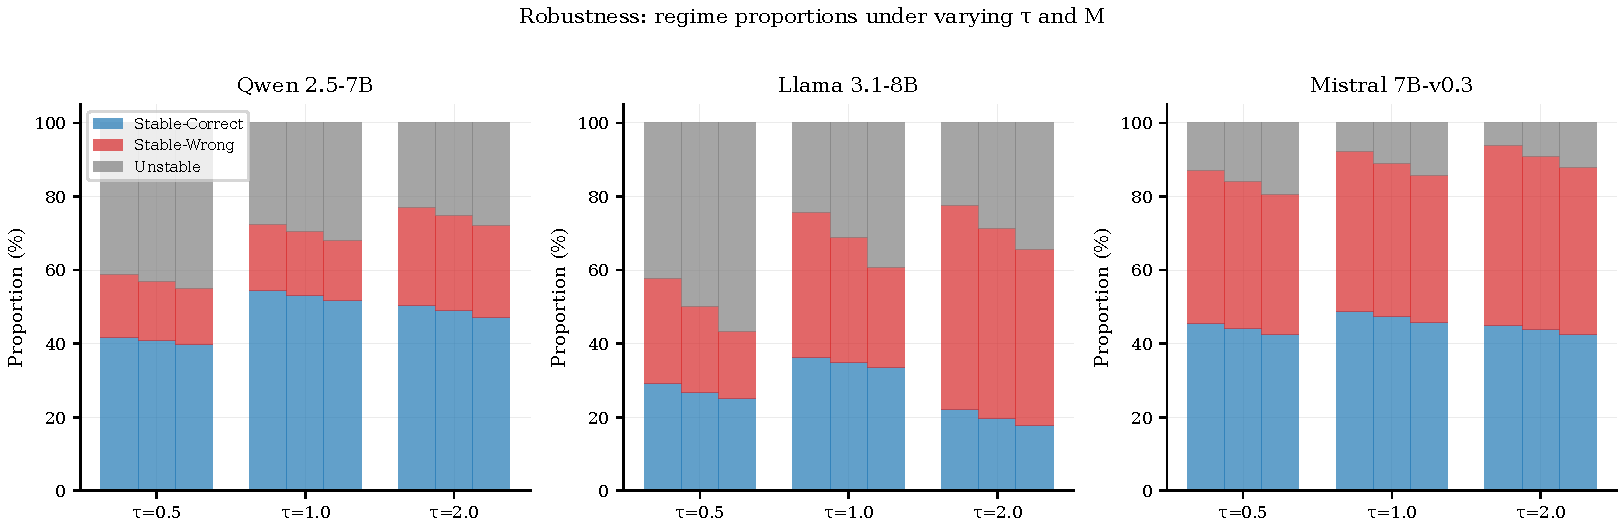
\includegraphics[width=0.95\textwidth]{figures/fig6_robustness.pdf}}
\caption{Regime proportions vary smoothly under hyperparameter perturbation.
Stacked bar charts of regime proportions for each model under $\tau \in \{0.5, 1.0, 2.0\}$ and $M \in \{0.5, 0.75, 1.0\}$.
No discontinuous jumps appear.
Stricter thresholds increase the Unstable fraction; softer margins dilute the Stable fractions slightly.}
\label{fig:robustness}
\end{center}
\end{figure*}


%% ============================================================
%% 5. LIMITATIONS
%% ============================================================
\section{Limitations}
\label{sec:limitations}

\begin{enumerate}
\item \textbf{Restricted four-choice readout.}
All analyses operate on four option-token logit scores.
The model's full vocabulary and internal hidden-state structure remain invisible.
The model may ``know'' an answer in a representation our four-token probe cannot detect.

\item \textbf{No mechanistic claims.}
This paper deliberately avoids causal claims about attention, MLP, or any internal circuit.
We report phenomenology: what the output trajectory looks like, not \emph{why} it looks that way.
Mechanistic attribution requires additional inference (activation patching, ablation) that is reserved for Part~II.

\item \textbf{Decision space is a proxy.}
The PCA trajectories in \cref{fig:pca} live in a four-dimensional option-score space, not in the high-dimensional hidden-state manifold.
This space captures the model's decision signal but not the full representational dynamics.

\item \textbf{Threshold conventions.}
$\tau = 1.0$, $M = 0.75$, and max flips $= 1$ \emph{define} regime boundaries rather than \emph{discovering} them.
\cref{sec:robustness} shows smooth degradation, but the partition is a convention.

\item \textbf{Scale.}
Only 7--8\,B models are studied.
Scaling behavior at 13\,B, 70\,B, or beyond is unknown.

\item \textbf{Format.}
Only four-choice multiple-choice; open-ended generation may differ.

\item \textbf{Single seed.}
All results from one deterministic run (seed 12345).
\end{enumerate}


%% ============================================================
%% 6. CONCLUSION
%% ============================================================
\section{Conclusion}
\label{sec:conclusion}

A transformer's decision on a multiple-choice question is not a point but a path.
By tracking four option scores across every layer, we defined a soft margin that smooths competitor-switching artifacts, classified trajectories into three regimes, and visualised the resulting dynamics in a decision space defined entirely by cached logit vectors.

Three findings stand out.
First, regime separation emerges gradually across depth: all regimes overlap at the embedding layer and separate by the final layer.
Second, commitment is a late phenomenon, concentrating in the last 20--30\% of depth for all three models.
Third, the regime structure is robust to hyperparameter perturbation, varying smoothly rather than discontinuously.

These results establish the phenomenology.
What \emph{causes} the observed trajectories---which components push toward or away from the correct answer---is the subject of Part~II, which will require additional inference.


%% ============================================================
%% IMPACT STATEMENT
%% ============================================================
\section*{Impact Statement}

This paper presents an observational analysis of existing model outputs.
It does not train models, generate text for consumption, or recommend deployment decisions.
We do not foresee specific negative societal consequences beyond those generally associated with advances in machine learning understanding.


%% ============================================================
%% REFERENCES
%% ============================================================
\bibliography{references}
\bibliographystyle{plainnat}


%% ============================================================
%% APPENDIX
%% ============================================================
\clearpage
\appendix

\section{Reproducibility Stamp}
\label{sec:appendix_reproducibility}

The data, code, and build process for this paper are fully specified.
The build script \texttt{build\_part1\_assets.py} reads cached parquet files, computes all metrics and figures, and writes a \texttt{BUILD\_INFO.json} file containing:
\begin{itemize}
\item The \texttt{parquet\_dir} path used.
\item SHA-256 hashes of every source parquet file.
\item The git commit hash at build time.
\item The build timestamp in UTC.
\end{itemize}

\noindent To reproduce:
\begin{verbatim}
HF_HUB_OFFLINE=1 TRANSFORMERS_OFFLINE=1 \
  python scripts/part1/build_part1_assets.py \
    --parquet-dir results/parquet \
    --output-dir paper/part1
\end{verbatim}

\noindent All random operations use \texttt{numpy.random.Generator} with seed~$12345$.
Grouping operations sort keys \texttt{(model\_id, prompt\_uid, layer\_index)} before iteration.


\section{Additional Robustness}
\label{sec:appendix_robustness}

\paragraph{Flip-count threshold.}
Setting \texttt{max\_flips} to 0 (stricter) reduces the Stable classes by approximately 5--8\% across models.
Setting it to 2 (looser) expands them by 3--5\%.
The qualitative regime structure is preserved.

\paragraph{Per-domain analysis.}
STEM domains show higher Stable-Wrong rates (confident factual errors).
Humanities show higher Unstable rates (ambiguous or context-dependent questions).
Social sciences are intermediate.
Domain-level regime proportions vary but the three-regime structure is present in every domain with $\geq 50$ prompts.

\end{document}
